\documentclass[11pt)]{beamer}
\usetheme{Copenhagen}

\defbeamertemplate*{headline}{split}
{%
  \leavevmode%
  \hbox{%
  \begin{beamercolorbox}[wd=.5\paperwidth,ht=2.65ex,dp=1.5ex,right]{section in head/foot}%
    \usebeamerfont{section in head/foot}\insertsectionhead\hspace*{2ex}
  \end{beamercolorbox}%
  \begin{beamercolorbox}[wd=.5\paperwidth,ht=2.65ex,dp=1.5ex,left]{subsection in head/foot}%
    \usebeamerfont{subsection in head/foot}\hspace*{2ex}\insertsubsectionhead
  \end{beamercolorbox}}%
  \vskip0pt%
}
\usepackage{subcaption}
\defbeamertemplate*{footline}{split}
{
	\leavevmode%
   	\hbox{%
      \begin{beamercolorbox}[wd=.5\paperwidth,ht=2.25ex,dp=1ex,center]{author in head/foot}%
        \usebeamerfont{author in head/foot}\insertshortauthor
      \end{beamercolorbox}%
      \begin{beamercolorbox}[wd=.4\paperwidth,ht=2.25ex,dp=1ex,center]{title in head/foot}%
        \usebeamerfont{title in head/foot}\insertshorttitle
      \end{beamercolorbox}%
      \begin{beamercolorbox}[wd=.1\paperwidth,ht=2.25ex,dp=1ex,right]{date in head/foot}%
        \usebeamerfont{date in head/foot}
        \insertframenumber{} / \inserttotalframenumber\hspace*{2ex}
      \end{beamercolorbox}}%
      \vskip0pt%
}

\setbeamertemplate{caption}{\raggedright\insertcaption\par}



\usepackage[utf8]{inputenc}
\usepackage{amsmath}
\usepackage{amsfonts}
\usepackage{amssymb}
\usepackage{graphicx}
\usepackage{lmodern}
\usepackage{color}
\usepackage{multirow}
\graphicspath{ {./figures/} }
\author{Judith Abécassis, Timothée Lacroix}
\title{SSL via Locally Sensitive Hashing (LSH)}
%\setbeamercovered{transparent} 
\setbeamertemplate{navigation symbols}{} 
%\logo{} 
\institute{Graphs in Machine Learning} 
\date{April 2015} 
%\subject{}
\AtBeginSection[]

\usepackage{tikz}
\usetikzlibrary{shapes,arrows,positioning}

\begin{document}
\graphicspath{{./../report/figures/}}
\begin{frame}
\titlepage
\end{frame}

{
  \begin{frame}
    \frametitle{Table of contents}
    \tableofcontents[currentsection]
  \end{frame}
}


\section{Challenge}
\begin{frame}{Classify a lot of elements in a SSL context}

		\begin{figure}
			\centering
			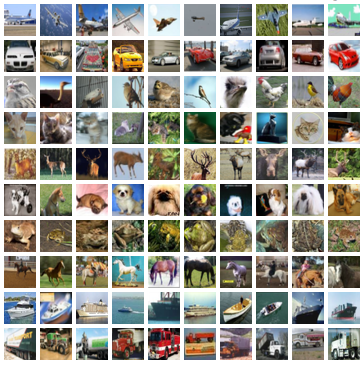
\includegraphics[width=\textwidth]{cifar-10.png}
			\caption{Crowd}
		\end{figure}


\end{frame}

\section{Semi-Supervised Learning Framework}
\begin{frame}{Leverage information from unlabeled nodes in the graph}

\end{frame}

\begin{frame}{The harmonic solution}
\end{frame}

\begin{frame}{Issues arise with the size of the graph}
\end{frame}

\section{Locality Sensitive Hashing}
\begin{frame}{Presentation of the principle}
\end{frame}

\begin{frame}{Accuracy}
\end{frame}

\section{Theory}
\begin{frame}{}
\end{frame}

\begin{frame}{Limitations to obtaining a bound for LSH}
\end{frame}

\begin{frame}{Empirical results on LSH accuracy}
\begin{itemize}
\item Instead of getting a theoretical bound, we have explored in a practical setting the error made by LSH
\begin{figure}[!h]
 \begin{subfigure}{0.27\textwidth}
   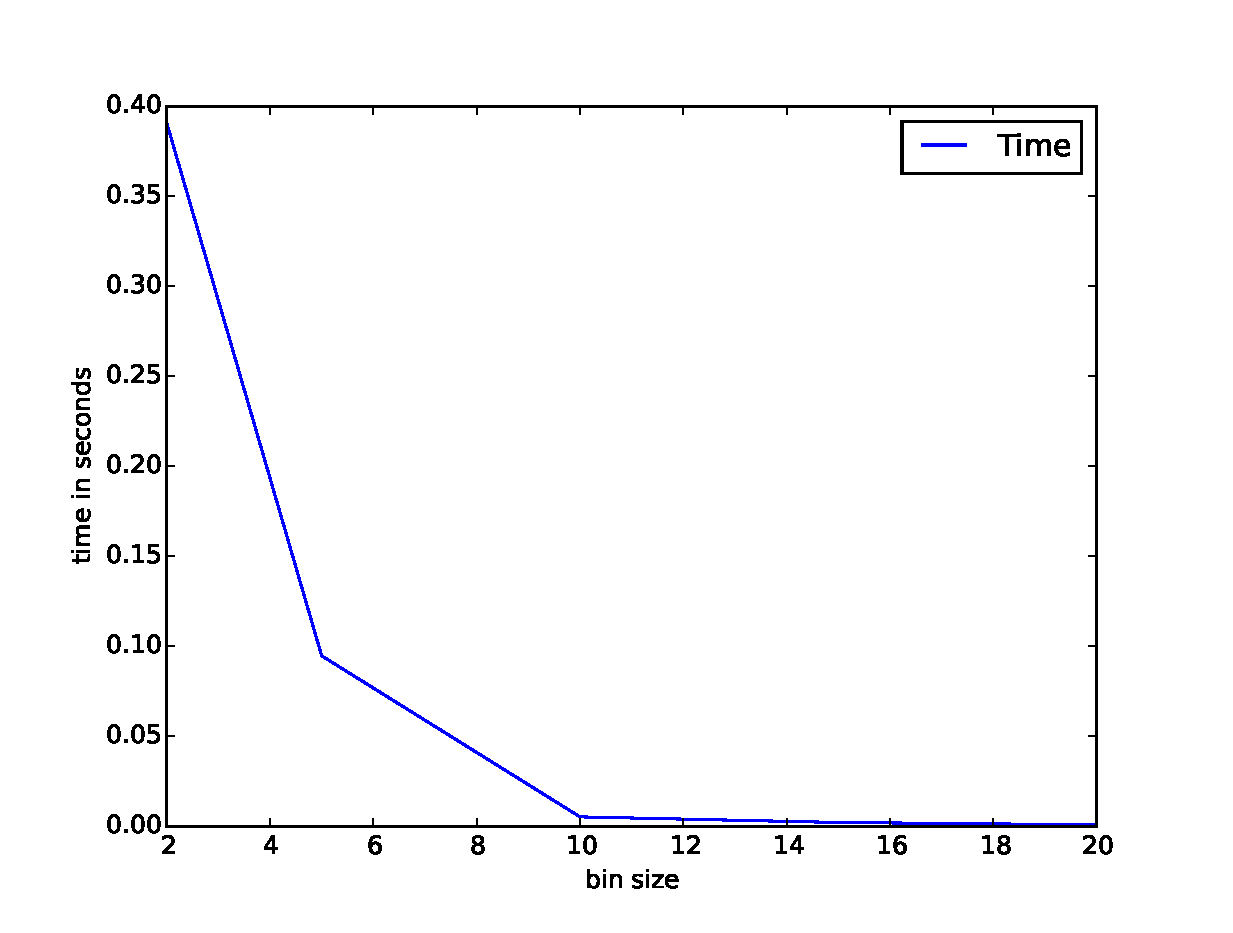
\includegraphics[width=\textwidth]{time_binsize.eps}
   \caption{Average time for a nearest neighbor query, as the number of bucket increases}
 \end{subfigure}\hfill
 \begin{subfigure}{0.27\textwidth}
   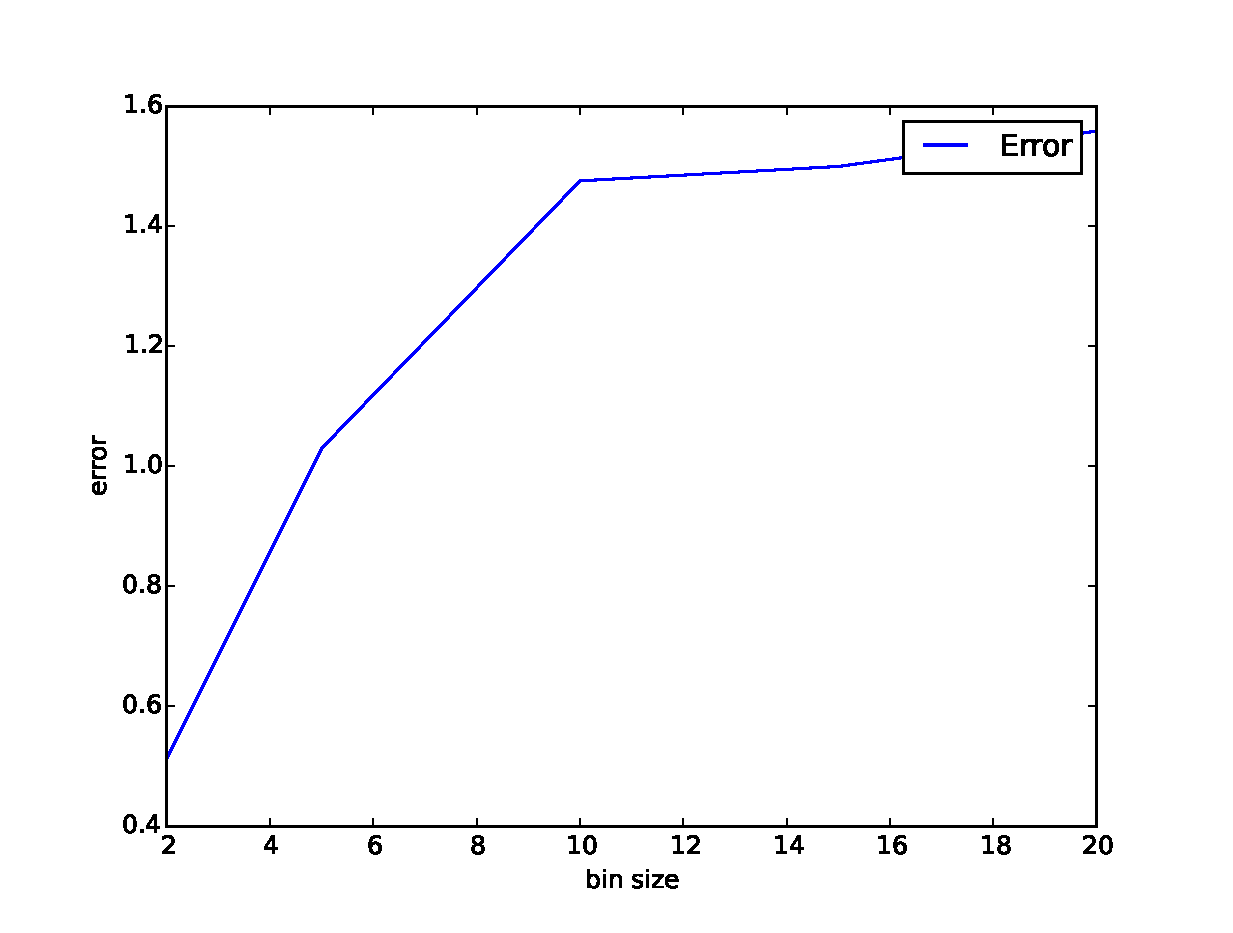
\includegraphics[width=\textwidth]{error_binsize.eps}
   \caption{Average normalized error for an approximated line of the Laplacian and an exact line, as the number of bucket increases}
 \end{subfigure}\hfill
 \centering
 \begin{subfigure}{0.27\textwidth}
   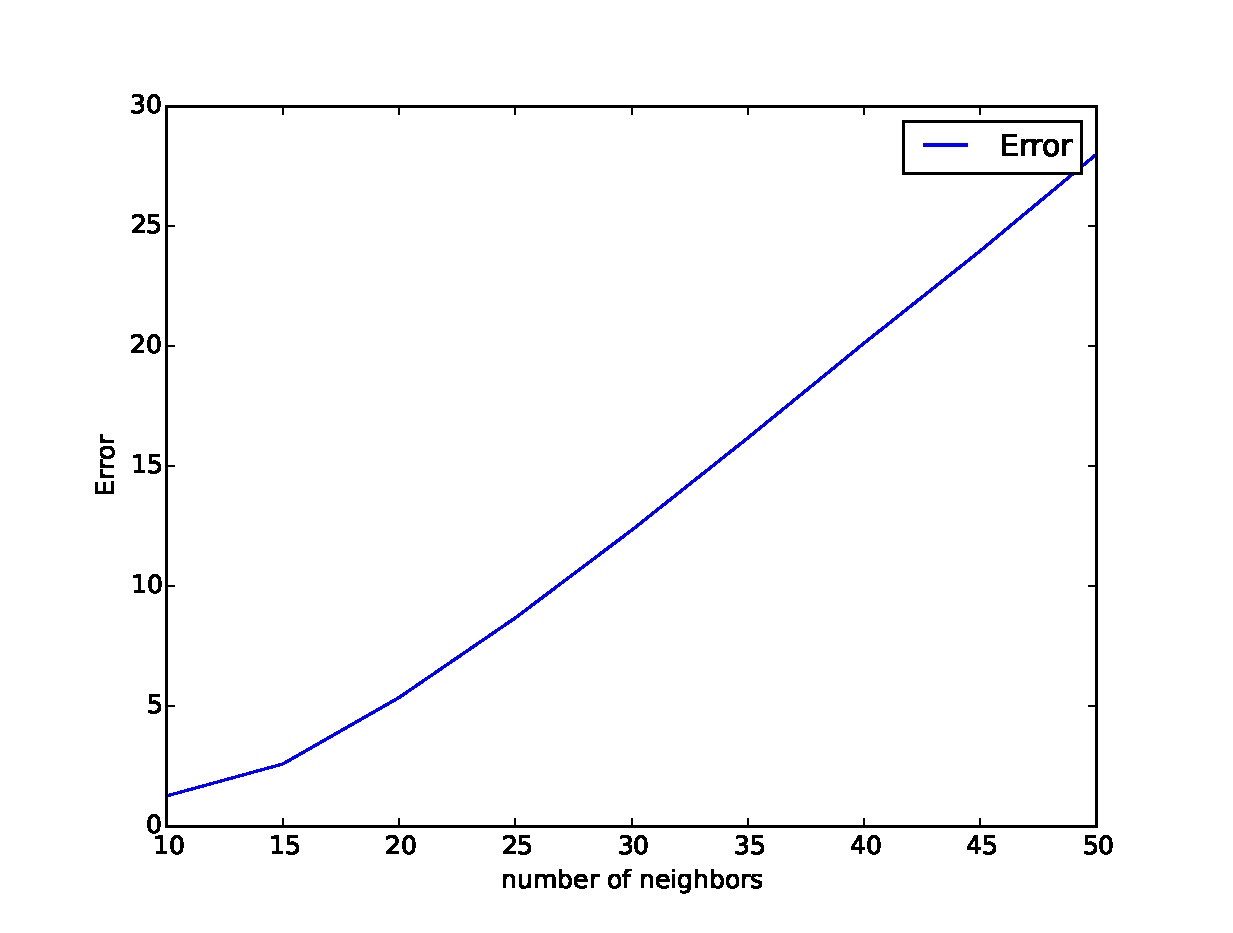
\includegraphics[width=\textwidth]{error_k.eps}
   \caption{Average normalized error for an approximated line of the Laplacian and an exact line, as the number of neighbor increases}
 \end{subfigure}

\end{figure}
\end{itemize}

\end{frame}

\section{Experiments}
\begin{frame}{The tinyImage dataset and preprocessing steps}
\begin{itemize}
\item ~80 million unlabeled images
\item CIFAR-100 labels: 10 classes with 600 labeled images in each
\item enriched with GIST descriptors (384 dimensions)
\item PCA on the 80M images: down to 32 dimensions
\end{itemize}
\end{frame}

\begin{frame}{Setting to assess performance}
\begin{itemize}
\item we consider $C$=10 random classes
\item for each class, we select $t$ positive and $t$ negative (in one of the remaining $100-C$ classes, $t\in \{0, 1, 2, 3, 5, 8, 10, 16, 20, 40, 60, 100\}$. Those are labeled nodes from the training set.
\item we compute the lerning step (by LSH+HFS or Fergus algorithm)
\item we select 100 positive test images and 200 negative ones for each of the $C$ classes (unlabeled)
\item we measure precision at 15 \% recall.
\end{itemize}
\end{frame}

\begin{frame}{Problems with LSH and GRaphlab implementations}
We have encountered several issued due to computation time while applying LSH+HFS method
\begin{itemize}
\item computation of the graph is long (~2600 sec)
\item one propagation step is long too (~1100 sec)
\end{itemize}
We have adapted the setting to save some computation time
\begin{itemize}
\item only positive and neutral labels (0 and 1s), to allow doing one propagation for the $C$ classes and not $C$ propagation steps
\item only consider the first 25 classes, and not 100 (otherwise it is even longer)
\end{itemize}

{\color{red}\textbf{Problem} results are no longer comparable to the Fergus baseline}

\end{frame}

\begin{frame}{Results}
\begin{figure}
  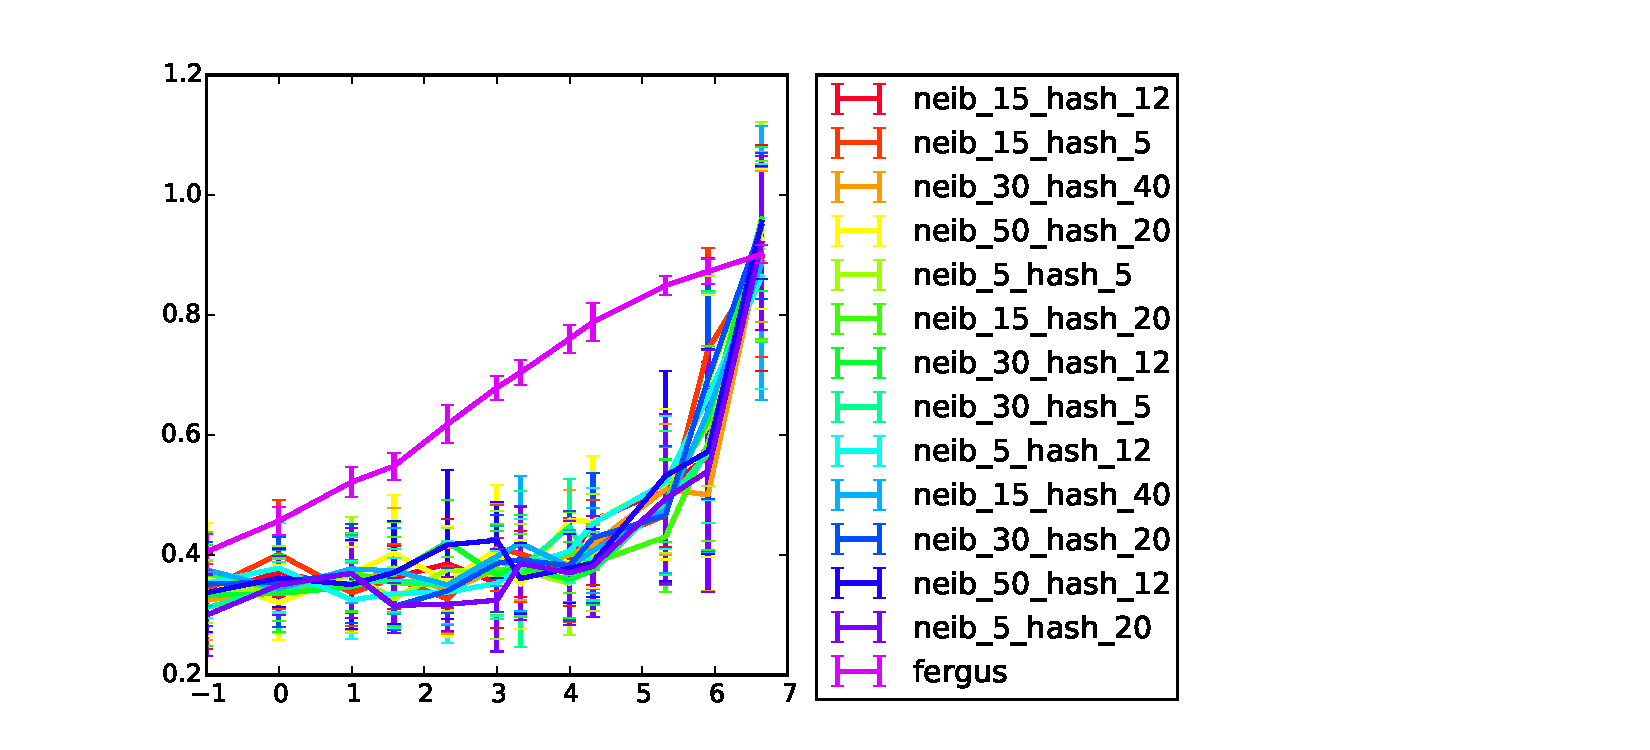
\includegraphics[width=\textwidth]{method_comp.pdf}
\end{figure}
\end{frame}

\section{Conclusion}
\begin{frame}{Conclusion}
\begin{itemize}
\item we have encourageing results on LSH performance
\item computational limitations of current implementation prevent from proper testing of LSH+HFS methodology
\end{itemize}
\end{frame}

\begin{frame}{Future work}
There are some variants of LSH method that learn hashing on data and could prove even more efficient.
\end{frame}











\end{document}